\chapter{COSMIC and Stellar Populations Synthesis}
The abundance of information of the electromagnetic spectrum allowed us to build highly detailed models of various celestial objects such as stars, both on their individual internal structure and on how this is influenced by the interaction with other bodies, for instance in binary systems.
In the pursuit of reaching a greater sensitivity in the gravitational counterpart too, which could potentially reveal new information, or place better constrains on the existing models, these stellar models, when combined with a good theory of gravity, can be used to construct synthetic populations that reproduce observable features like luminosity, color, and chemical composition, which could enable us to predict what their gravitational signal would look like.
In gravitational waves research, our observational capabilities are still very limited, and the signals are still comparatively very weak relative to their electromagnetic counterpart. 
Thererfore, methods that rely on simulations can be very useful both to  explore how different sources could look like in the gravitational wave domain, and how effectively they could be detected with current or future instruments.

\section{Stellar populations synthesis codes}
Generating a synthetic population of stars is a very complex task, that involves multiple steps, each involving important choices.
\textit{First}, we need to choose a starting point: we could start from the very beginning of stars formation and simulate all the process from the birth onward, or we could select a later phase in the stars evolution, shared from the most, in order to reduce unnecessary computational power and time consumption. 
If we want to simulate entire stellar populations choosing a starting point also implies selecting appropriate distributions for the main parameters that characterize the "starting point population", like masses, metallicities, but also orbital parameters for the stars that are in binary systems, like orbital period, distance, and eccentricity. 
\textit{Second}, we must choose how the stars will evolve from the starting point, and this involves the single star evolution but also the effects that interaction with other stars in binary systems have on it.
\textit{Finally}, we have to decide when we want to stop the simulation, choosing an endpoint that aligns with the needs of this study.

\subsection{The starting point}
As we know, in the Hertzsprung-Russel diagram, which plots the \textit{luminosity} of the stars vs their \textit{color index}, most of the stars appear distributed in the \textbf{main sequence} (\textbf{MS}), a continuous and distinctive band.
A star's position on this band is determined by its initial mass, and a good rule of thumb is that the most massive stars are hotter, more luminous, and evolve more quickly, while the lower-mass stars burn their fuel more slowly, and remain on the MS longer.
\begin{figure}[h!]
    \begin{center}
        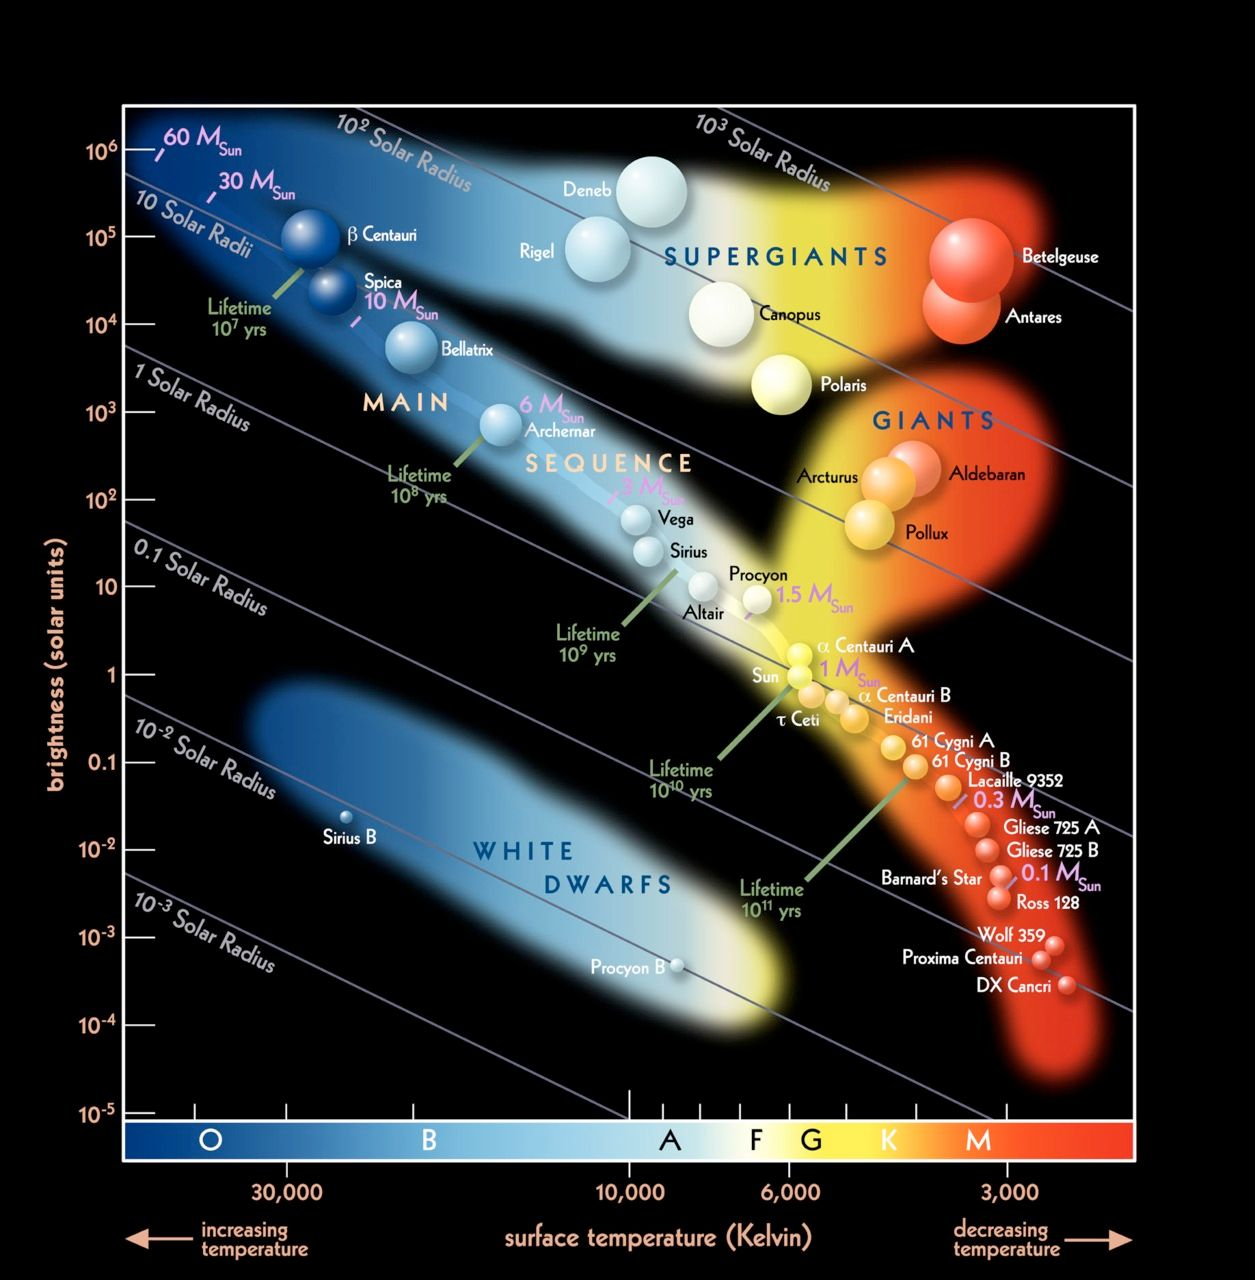
\includegraphics[width=0.65\textwidth]{images/Hertzsprung_Russel_Diagram.jpg}
    \end{center}
    \caption{WRITE CAPTION, INSERT REFERENCE}\label{fig: Hertzsprung_Russel_Diagram}
\end{figure}\\
Since almost all stars go through a phase in the MS, and evolve from there differently, in this work, the chosen starting point for stellar evolution is the Zero Age Main Sequence (ZAMS). 
At this stage, stars have just begun hydrogen burning in their cores, marking the start of their stable main sequence phase.
This allows to bypass the early phases of star formation, which are much less relevant to the gravitational wave sources of interest, while still capturing the essential evolutionary processes that lead to the formation of compact objects.

\subsection{Single star evolution}
Simulating the evolution of a single star is in itself a very complex matter, and the only way to make it computationally feasible in the context of large-scale population synthesis is to approximate the evolution for a wide range of mass $M$ and metallicity $Z$. 
In fact, detailed evolution codes can require substantial computational time even for the evolution of a single star, which is not practical when generating a full-scale astrophysical population containing millions of stars. 
Also, in order to make population synthesis statistically robust a large enough number of stars of a certain type must be evolved in order to overcome stochastic noise (in particular, the Poisson noise for $n$ simulations of a particular type of star, implies an error that grows as $\sqrt{n}$).
A winning strategy, adopted by several population synthesis frameworks, is to pre-generate a large grid of detailed stellar evolution models, and use them to derive a number of interpolation formulae as functions that approximate stellar properties as a function of age, mass and metallicity. 
In \cite{SSE} this method is implemented through the development of a set of \textbf{Single Star Evolution} (\textbf{SSE}) formulae, with the result of a very compact, efficient and adaptable code, which makes it perfect for the integration of binary-star interactions.
The work presented in \cite{SSE} therefore serves as the theoretical and computational foundation for many complex stellar population synthesis codes, including the one used in this thesis. It takes care of the single-star evolution of stars from ZAMS through all the possible evolutionary outcomes, depending on the star's initial conditions.

\subsection{Binary stars evolution}
While the evolution of single stars already represents a challenge, the inclusion of binary interactions introduces a much higher level of complexity.
In such systems, the evolution of each star is strongly influenced by its companion through a variety of processes, such as mass transfer and accretion, common envelope evolution, collisions, supernova kicks, tidal effects, angular momentum loss, and mergers.
These interactions can drastically alter the final outcomes, and are essential for modeling the formation of compact binaries that are potential gravitational wave targets for LISA.
To efficiently model binary evolution within the framework of stellar population synthesis, the work of \cite{BSE} extends the SSE formalism by introducing a set of prescriptions for binary interactions, and updating the treatment of processes such as Roche lobe overflow, common envelope evolution ans coalescence by collision, leading to the development of the \textbf{Binary Star Evolution} (\textbf{BSE}) algorithm.
This code includes the interpolation-based approach used in SSE for single-star evolution, but adds a comprehensive treatment of binary-specific processes, enabling the simulation of a wide range of binary configurations but keeping the affordable computational requirements of SSE.
The BSE algorithm tracks the joint evolution of both stars in a binary system, taking into account their initial parameters, such as masses, orbital period, eccentricity, and metallicity, and updates these properties dynamically as the system evolves.
The flexibility and speed of the BSE code make it a key component in many modern population synthesis tools, including the one used in this thesis, which we will now introduce.

\section{COSMIC}
For the purposes of this work, we employ a community-developed binary population synthesis (BPS) python-based code, called the \textbf{Compact Object Synthesis and Monte Carlo Investigation Code} (\textbf{COSMIC}), whose <<\textit{primary purpose is to generate synthetic populations with an adaptive size based on how the shape of binary parameter distributions change as the number of simulated binaries increases}>>
\footnote{\url{https://cosmic-popsynth.github.io/docs/stable/pages/about.html}}. 
COSMIC's binary evolution is built upon BSE, incorporating extensive modifications in order to include updated physical prescriptions.
It  includes all necessary tools to generate a population, from the generation of initial conditions, to scaling the simulated systems to full-scale astrophysical populations.
The code is presented in \cite{Breivik}, where it is described in full detail and used, as a proof of concept, to simulate the Galactic population of compact binaries and their associated gravitational wave signal.
In the following section we will see the main features of the code, and explain what makes it the right choice for this thesis work.

\subsection{Fixed population}
A fundamental concept in COSMIC, which is the key to the code's efficiency, is the idea of \textit{fixed population}.
This refers to a relatively small sample of just enough binaries to capture, in a statistically meaningful way, the underlying shape of the parameter distribution functions of the target population, as determined by the user specified Star Formation History (SFH) and evolution model.
This is achieved following an iterative process designed to reach a convergence with respect to a defined matching condition, and consists of five key steps:
\begin{enumerate}
    \item The user selects a binary evolution model and SFH;
    \item Based on the SFH and the chosen initial parameter distribution, an initial population is generated;
    \item The population evolves for a user specified number of steps, according to the selected evolution model;
    \item If it is the first iteration, half of the simulated systems is compared with the total population. In the following steps, the population from the previous one gets compared to the population containing both the current and previous iterations.
    In any case, the comparison is done in order to check if the matching condition has been achieved;
    \item Once the parameter distributions of the population have converged, the corresponding population is called \textit{fixed population}, which represents the statistical features of a binary evolution model.
\end{enumerate}
In practice, the fixed population is the converged, computationally efficient representation of the systems that we want to simulate, embedded in a complete small-scale synthetic galaxy that also contains other stellar components.
The output is stored in a data frame, which separates the full galaxy properties from the fixed population ones.
The last step that is required to construct a full size astrophysical population is to scale the fixed population (by mass or by number of stars) with a re-sampling approach with replacement, allowing to extrapolate a larger final population that preserves the statistical properties encoded in the fixed population.





- COSMIC pipeline (why it's quick, intro to fixed population idea, match conditions, ...)
- important parameters in COSMIC (the ones user chooses - stress on metallicity relevance)
- population's parameters (the ones COSMIC gives to user)
    - parameter distribution graphs
- Scaling to astrophysical population, what is needed (refer to next chapter
